\documentclass[12pt,a4paper]{article}

% Codificación e idioma
\usepackage[utf8]{inputenc}
\usepackage[T1]{fontenc}
\usepackage[spanish,es-nodecimaldot]{babel}
\usepackage{lmodern}

% Formato y composición
\usepackage{geometry}
\usepackage{setspace}
\usepackage{microtype}
\usepackage{csquotes}
\usepackage{enumitem}
\usepackage{graphicx}
\usepackage{float}
\usepackage{placeins}
\usepackage{caption}
\usepackage{amsmath,amssymb}
\usepackage{tikz}
\usetikzlibrary{decorations.pathreplacing}
\usetikzlibrary{positioning,arrows.meta,babel}
\usepackage[hidelinks]{hyperref}

% Citación clásica BibTeX
\usepackage[round,authoryear]{natbib}

\geometry{margin=2.5cm}
\setstretch{1.15}

\title{Fragmento de tesis de licenciatura \textit{La conciencia interna del tiempo en la fenomenología de Husserl y su relación con  la individuación de la conciencia y la constitución de sentido}}
\author{Valeria Montjoy Bustamante}
\date{Setiembre 2025}

\begin{document}

\maketitle

% Se conserva la numeración 1.3 del fragmento original de la tesis.
\setcounter{section}{1}
\setcounter{subsection}{2}

\subsection{La estructura básica del ahora: \textit{duración} como condición de posibilidad de la temporalidad de las vivencias}\label{sec:estructura-ahora}

\begin{quote}
``El tiempo es rígido y, con todo, el tiempo fluye''
\end{quote}

\cite[§31, p.~84]{husserl2002}

El ahora, como rasgo esencial, posee un carácter de presencia total. El
ahora se presenta como el momento que siempre está marcando el reloj.
Cuando hablamos del ahora, solemos pensar en este como el momento más
``real'', incluso, como lo ``único que existe''. Dejamos fuera de él lo
que ya ha pasado o todavía no pasa, ya que se diferencian claramente
respecto al ahora. Por más que el ahora irreflexivamente se presente
como el punto temporal en el que siempre estamos, podemos afirmar que
todo ahora posee un horizonte temporal en relación necesaria con lo
pasado y futuro. Si no fuera así, viviríamos en un \emph{eterno
presente,} lo cual impediría el despliegue temporal necesario para la
multiplicidad de vivencias conscientes. El paso de un ``ahora'' a otro
sería un salto abismal, como la infinidad de decimales que hay entre el
1 y el 2. Si todo ``ahora'' que ocurre no demanda un horizonte temporal
de pasado y futuro, no sería posible distinguir la multiplicidad de
puntos temporales que se enumeran en el tiempo objetivo. No podemos ver
la hora en el reloj sin esta continuidad entre el momento que acaba de
pasar y el que va a suceder. Para poder ``dar'' la hora en cada momento
marcado numéricamente, ya se debe de suponer una duración continua que
el tiempo objetivo no muestra en el paso de un instante a otro, sino que
presupone.

Las consecuencias de la comprensión discreta del tiempo se pueden
encontrar en los estudios de Franz Brentano, maestro de Husserl, quien,
para explicar cómo podemos tener una noción de la temporalidad de
nuestros actos perceptivos recurre a la fantasía para explicar cómo
podemos sintetizar, unir o \emph{asociar} distintos momentos de
captación \cite[p.~54]{mensch2010}. Mediante el acto de la fantasía podemos
``ampliar nuestra intuición temporal'' y proyectar vivencias al pasado o
futuro de diferentes fenómenos psíquicos:

\begin{quote}
``\ldots Toda clase de deseos y actos de voluntad, así como las
convicciones y opiniones de todo tipo, y una amplia gama de
representaciones que tienen su origen en la fantasía. De todos los
fenómenos psíquicos, únicamente las sensaciones --y ni siquiera todas
ellas-- permanecen dentro del ámbito de lo mensurable'' \cite[p.~52]{brentano2009}\footnote{Traducción de la versión en inglés}.
\end{quote}

Brentano recurre a explicar los procesos asociativos de vivencias a
través del acto de la fantasía para explicar la relación de la
percepción presente con vivencias pasadas y futuras: ``Brentano, por lo
tanto, atribuye la conjunción a un proceso de `asociación primordial'
por el cual la fase pasajera de una apariencia se une a la fase ahora
como una `idea de fantasía'\,'' \cite[p.~188]{morrison1970}. Husserl, como
veremos, no busca recurrir a otros actos conscientes para explicar la
asociación de múltiples vivencias, sino describir una estructura
temporal que atraviesa todo acto. Esto hace que la temporalidad no sea
producto de la percepción consciente, sino que esta última necesite de
una estructura temporal para articularse.

Los exámenes fenomenológicos de la conciencia interna del tiempo
muestran cómo cada vivencia actual se extiende en distintas fases que le
dan una continuidad temporal y entrelazan con el horizonte de vivencias
pasadas y futuras. Dicha continuidad de la temporalidad interna de la
conciencia explica la duración temporal de cada acto y de la vida
consciente en su conjunto sin recurrir a una noción discreta de tiempo
que comprende al ahora como un instante aislado en una serie lineal de
sucesiones. Brough comenta que la captación de la duración del ahora
descrito en los exámenes fenomenológicos del tiempo de la conciencia
demuestra que incluso nuestro lapso o duración de tiempo más ``corta''
posee más fases que el instante puntual en cada momento sustituido por
uno nuevo:

\begin{quote}
Así que incluso en el momento presente ocurre una cierta indecidibilidad
entre uno y muchos, y con la comprensión metafísica del tiempo como una
sucesión lineal de momentos del ahora, el momento realmente presente se
encuentra acompañado por miradas de otros momentos que lo preceden o lo
siguen. Cada uno puede ser una unidad considerada en sí misma, pero el
punto es que ninguno de ellos por sí mismo podría componer el
tiempo---el tiempo exige que haya muchas de tales unidades---y así se
compromete el valor de la mera presencia de un sólo momento. La
comprensión del momento por parte de Husserl es quizás menos
pirotécnica, pero ciertamente es sutil e introduce en el ahora un
sentido más profundo de indecidibilidad \cite[p.~517]{brough1993}.
\end{quote}

En contraste con el tiempo objetivo, sujeto a una discreción lineal de
instantes que pueden ser numéricamente medidos, Husserl expone que la
temporalidad consciente no se reduce a una serie de instantes, sino que
consiste en una duración que implica siempre la distinción de fases que
corresponden a lo ya pasado, a lo presente y lo anticipado. Limitaciones
de una mirada discreta del tiempo se muestran al reflexionar sobre
cualquier vivencia, por ejemplo, el oír una melodía o hablar. Cuando
recuerdo dichas vivencias, no recuerdo la suma de notas o de sílabas
pronunciadas sucesivamente, sino que recuerdo la unidad desplegada de la
melodía o las palabras. Originalmente, el tiempo se da en esta unidad
constitutiva de toda experiencia. La comprensión discreta del tiempo, si
bien puede lograr una exactitud y utilidad para propósitos de medición o
cálculo de fenómenos, es una aproximación artificial, no intuitiva, al
tiempo, ya que no da cuenta del fenómeno original de la continuidad
temporal con la que captamos objetos que, bajo una determinada mirada
científica, podemos medir\footnote{Para Husserl, un rasgo esencial de la
  intuición del tiempo que este se dé en una duración: ``Lo que sí
  pertenece a la esencia de la intuición de tiempo es, en cambio, el ser
  a cada punto de su duración (que nosotros podemos convertir
  reflexivamente en objeto) conciencia de \emph{lo que acaba de ser} y
  no mera conciencia del punto de ahora del objeto que aparece durando''
  (Husserl 2002, §12, 54). La duración, en contraste con la mera
  presencia, nos abre el camino a examinar cómo lo que está presente se
  constituye a partir de lo que no lo está, ya sea porque \emph{ya no
  es} o porque \emph{todavía no lo es.}}.

Se exige la distinción de tres momentos temporales: el ``ahora
puntual'', el ``ahora-reciente'' y el ``ahora-adveniente''. Estos tres
momentos se constituyen en la misma conciencia inmanente, la cual el
fenomenólogo examina en las vivencias y puede distinguir en la
conciencia una duración que no es discreta sino continua. Son momentos
enteramente abstractos y se les introduce en la descripción de la forma
en la que se articula la duración mínima. La duración inmanente se
muestra a la mirada del fenomenólogo como un flujo continuo de
vivencias, como una duración de duraciones \cite[p.~120]{husserl2002}. Así, los
tres momentos que se distinguen son enteramente abstractos: cada ahora
puntual está a la vez abierto hacia adelante y adherido hacia atrás.
Correlativamente a estos fenómenos, el fenomenólogo distingue los
momentos de la propia conciencia de tiempo inmanente. Esta
pre-estructura noético-noemática, de los momentos del ahora puntual, el
ahora adveniente y el ahora-reciente es anterior a toda constitución de
tiempo objetivo. Yo puedo \emph{medir} la cantidad de tiempo (objetivo)
que tarda un lápiz de caer al piso desde la mesa. Sin embargo, esta
medición \emph{supone la vivencia} de la percepción de la caída del
lápiz que se despliega en una duración temporal. Así, el ``ahora''
cumple una función tanto en el tiempo objetivo como en la temporalidad
interna de la conciencia. Yo puedo saber que ahora son las 11:00 am
porque el reloj está sucesivamente contando la serie de instantes
pasados y futuros para poder, en cada momento, apuntar al ahora. Sin
embargo, la conciencia del ahora se distingue porque \emph{no marca} un
ahora puntual, sino que todo momento \emph{vivido} implica una
estructura tripartita de duración. De este modo, la distinción de las
fases de la conciencia del ahora, sin embargo, no debe ser entendida
como una \emph{separación} sucesiva de instantes discretos: se dan más
bien \emph{como una unidad en cada} vivencia:

\begin{quote}
Del fenómeno decursivo sabemos que es una continuidad de constantes
mudanzas que forma una unidad inseparable; inseparable en trechos que
pudiesen existir por sí, e indivisible en fases que pudiesen existir de
por sí, en puntos de la continuidad. Los fragmentos que nosotros
abstractamente destacamos sólo pueden existir en el decurso íntegro, y
lo mismo las fases, los puntos de la continuidad decursiva (Husserl
2002, §10, 51).
\end{quote}

En otras palabras, la conciencia puede reflexionar sobre su propio
discurrir temporal, que muestra su unidad debido a la estructura
temporal encontrada en el ahora y que se distingue del tiempo objetivo
en el que discurren los objetos captados en la actitud natural. Así,
puede cambiar de objeto percibido, de acto mediante el cual lo aprehende
y su contenido y, sin embargo, su unidad es asegurada por esta cadena
estructurada de fases temporales que conectan toda vivencia pasada
presente y futura de la cual se pueda tener experiencia. La distinción
de las fases temporales de la conciencia del ahora muestra que el tiempo
interno de la conciencia es una temporalidad compleja, que no se
constituye a partir de instantes homogéneos en una sucesión lineal, sino
que, toda duración temporal implica una distinción de lo ya pasado, lo
presente y lo adveniente. Esto se corrobora al examinar cómo los
exámenes de la conciencia del tiempo se modifican con el avance de sus
exploraciones fenomenológicas, ya que las funciones de las fases de
retención y protención cobran una mayor relevancia ``Los cambios en el
diagrama\footnote{El diagrama se expondrá en la siguiente parte.} y su
descripción reflejan el cambio de enfoque de Husserl hacia los dos
sistemas de protenciones y retención y lejos de la zona de
actualización'' \cite[p.~135]{rodemeyer2003}.
\subsubsection{La estructura temporal de la conciencia del ahora: impresión originaria, retención y protención}\label{sec:estructura-tripartita}

Sin ir más lejos, pasemos a examinar la estructura tripartita inmanente
de la conciencia del ahora: la impresión originaria, la retención y la
protención con los momentos correlativos captados en estas: el ahora
puntual, el ahora-reciente y el ahora-adveniente: `` \ldots Sobre
cada `ahora' es la estructura `protoimpresión-retención-protención' de
la conciencia absoluta la que articula el darse de lo temporal. Esta
opera como una estructura invariante'' \cite[p.~251]{kretschel2014}. La mirada
natural del tiempo objetivo presupone este desdoblamiento de la
temporalidad consciente, lo que quiere decir que todo presente marcado
por el tiempo objetivo necesita darse en el horizonte de un antes y
después. Para yo saber que dar una vuelta por el parque con mi mascota
me toma de las 11:30 hasta las 12:00, es decir, para poder trazar una
secuencia de tiempo objetivo, implícitamente debo captar un horizonte de
momentos pasados y futuros a partir del instante actualmente marcado
objetivamente. Condición de posibilidad para captar y delimitar el lapso
temporal de los sucesos espacializados es que la propia conciencia ya es
una duración temporal de vivencias de dichos objetos. Sólo porque dichas
vivencias poseen una duración temporal en la cual fenomenológicamente se
pueden distinguir las fases que marcan las direcciones temporales de
presente, pasado y futuro, es que se puede comprender la sucesión de
momentos de tiempo objetivo. Pero este, al nivelar todos los instantes
como una serie de puntos homogéneos, no puede captar la distinción
esencial de temporalidad inmanente entre ellos.

Es necesario notar que la estructura del tiempo inmanente de la
conciencia no se da en el tiempo objetivable en el modo en que se dan
nuestras vivencias particulares, ya que esto nos llevaría a una
regresión infinita \cite[p.~86]{zahavi2010}\footnote{Esto quiere decir que el
  acto mismo debe de poseer ciertas estructuras que condicionen toda
  vivencia presente, pasada y futura, posibilitando que la conciencia
  pueda volver a ellos reflexivamente por su continuidad temporal. La
  conciencia no solo trasciende hacia objetos externos a ella, sino que
  puede reconducir su ``mirada'' hacia sus mismos actos y examinarlos
  aunque no con el mismo sentido de objetividad: podemos volvernos hacia
  todo acto en el horizonte temporal de la vida consciente. Todo acto de
  la conciencia posee la posibilidad de ser reflexivo, es decir, de
  poder volver sobre mis propias vivencias. Esto es característico de
  los actos noéticos y marca un contraste con los objetos dados. Por
  dicha estructura temporal de la conciencia, se muestran los diferentes
  niveles del acto consciente que entran en juego en toda vivencia
  intencional y que unifican en toda experiencia vivida la temporalidad
  de la conciencia con la temporalidad objetiva. ``La afirmación no es
  que el objeto de experiencia siempre debe diferir ontológicamente del
  sujeto de experiencia, como si el sujeto y el objeto de experiencia
  debieran ser necesariamente dos entidades diferentes. Más bien, la
  afirmación es simplemente que la experiencia en sí misma no se
  experimenta de forma prerreflexiva como un objeto \ldots. Lo que
  esto significa, sin embargo, es que sería un error concebir la
  relación entre la conciencia interna del tiempo y la experiencia
  intencional como si fuera una relación objetivante entre dos
  dimensiones distintas de la conciencia'' \cite[p.~332]{zahavi2010}.}. La
estructura temporal de la conciencia es lo que nos permite captar el
devenir temporal de nuestras vivencias y, por lo tanto, ella misma no
puede estar sometida a dicho devenir. No hay instancia anterior a ella
para captar el devenir temporal y, por lo tanto, todo análisis
fenomenológico del tiempo supone dicha estructura para que sea posible
la captación de una vivencia en general. El tiempo como ``algo''
distinguible la conciencia no es comprensible dentro de un análisis
fenomenológico: el tiempo se da en el terreno de la vida consciente.
Separar la estructura esencial de la conciencia del ahora de la
temporalidad objetivada es necesario para comprender la posibilidad de
la reflexión sobre las vivencias. Si bien las vivencias se pueden
objetivar al reflexionar sobre ellas, eso no significa que \emph{sean}
objetos o que aparezcan inicialmente como objetos, sino que, en tanto
\emph{vivencias,} se manifiestan en primera instancia como \emph{vividas
desde mí} e in-objetivables como cosas \emph{dadas}, pero \emph{pueden
volverse} objetos de la conciencia si es que esta se vuelve a ellas a
partir de un acto reflexivo que surge en su horizonte temporal. Esta
distinción fenomenológica evita una bifurcación ontológica radical entre
la vivencia y el objeto dado, ya que la vivencia no es un objeto como
los objetos intencionales dados en ellas, sino que se objetiva en el
mismo horizonte temporal en el que fue dada. Para poder reflexionar
sobre la estructura temporal de mis propias vivencias, no necesito
suspender el discurrir temporal mismo, sino distinguir, en él, las fases
esenciales intrínsecas a toda vivencia.

Husserl caracteriza a las vivencias examinadas en su duración temporal
como ``fenómenos decursivos'', ya que captamos la continuidad de
constantes mudanzas que ``forma una unidad inseparable; inseparable en
trechos que pudiesen existir por sí, e indivisible en fases que pudiesen
existir por sí, puntos de la continuidad'' \cite[§10, p.~50]{husserl2002}. Al
dirigir nuestra mirada a las vivencias en su duración temporal, lo que
captamos es un curso continuo de mudanzas que contienen captados a los
instantes puntuales del tiempo objetivo que medimos en la actitud
natural. Por eso, ``los fragmentos que nosotros abstractamente
destacamos sólo pueden existir en el decurso íntegro, y lo mismo las
fases, los puntos de la continuidad decursiva'' (Husserl, 2010, §10,
50). En otras palabras, la condición de posibilidad de toda captación de
tiempo, ya sea cuando contamos el tiempo objetivo del reloj o cuando
subjetivamente percibimos su paso, es captar una duración unitaria que,
al examinarla, nos muestra un tránsito constante de fases temporales que
indican las direcciones de pasado, presente y futuro. Antes de cualquier
referencia objetiva o subjetiva al tiempo, hay una estructura esencial
de duración temporal operando en toda vivencia consciente. Si bien estas
fases muestran el discurrir constante de la duración temporal, ``podemos
decir con evidencia que es en cierto modo inmutable en su forma''
\cite[§10, p.~50]{husserl2002}. Husserl busca notar el doble carácter de
multiplicidad y unidad del examen de la duración temporal de las
vivencias conscientes: por un lado, es una sola duración que captamos,
pero en dicha duración se muestra un discurrir constante de fases
temporales que es invariable en su estructura esencial de impresión
originaria-retención-protención que, por lo tanto, no está sometida ella
misma a un devenir temporal, sino que se mantiene invariable en toda
vivencia examinada.

En ese sentido, la conciencia puede captar su temporalidad volviéndose
sobre sus propios actos y las estructuras que lo condicionan separando
dicho análisis del objeto dado en las vivencias. Es esta estructura
temporal de la conciencia del ahora la que posibilita el sentido de lo
pasado, presente y futuro en la continuidad de la vida consciente y que
el tiempo objetivo supone en la sucesión de instantes. Ahora, pasemos a
examinar el gráfico que presenta Husserl en el parágrafo 10 de las
\emph{Lecciones}\footnote{Husserl, 2002, §10, 50.}:

\begin{figure}[htbp]
    \centering
    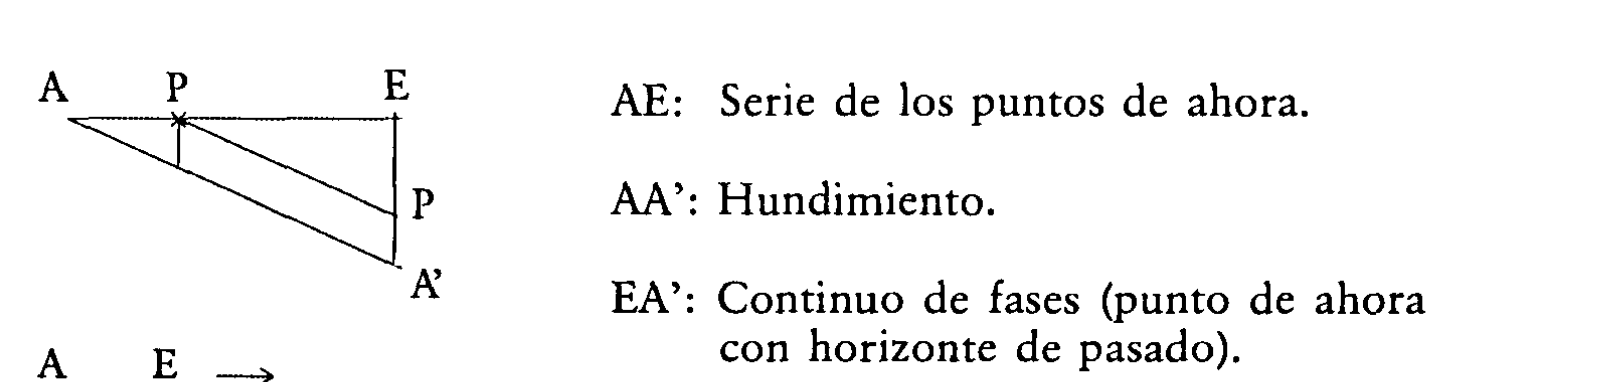
\includegraphics[width=0.88\textwidth]{figuras/diagrama_husserl_original.png}
    \caption{Diagrama de la conciencia interna del tiempo presentado por Husserl en el §10 de las \textit{Lecciones}.}
    \label{fig:diagrama-husserl}
\end{figure}

Husserl no desconoce la puntualidad irreductible del ahora. Este
carácter puntual es lo que denominamos ``instante'' en referencia al
tiempo objetivo y que en la conciencia interna del tiempo corresponde
directamente a un momento abstracto de la fase o duración. Lo que
permite la descripción de la duración de la conciencia del ahora es
comprender la estructura que permite la captación temporal de toda
vivencia en sus fases de impresión originaria-retención-protención. La
línea horizontal marca esta serie de \emph{ahoras} puntuales (AE)
captada como una continuidad constante. Estos, claramente, no se dan
simultáneamente, sino que se caracterizan por una continuidad que forma
la duración temporal. Asimismo, como vemos, esta no es una línea
horizontal, sino que posee puntos verticales que indican el hundimiento
de los puntos retenidos en el punto actual, lo cual muestra que la
duración temporal de la conciencia del ahora posee una profundidad
formada por los puntos temporales dejados atrás. El punto A no
desaparece, sino que se va hundiendo hasta ser un A', es decir, que es
retenido en el punto E a medida que el ahora sigue discurriendo y que
permanece constante en todo punto adveniente. Esta transformación del
ahora puntual a partir de una continuidad de momentos re-tenidos y
pro-tenidos, de ahoras recientes y ahoras advenientes estructura la
conciencia interna del tiempo.
\subsubsection{Los objetos temporales}\label{sec:objetos-temporales}

Husserl cree conveniente usar de ejemplo la percepción de un sonido, en
lugar de un objeto que aparece con una presencia más constante o
invariable, como una mesa, ya que por su aparente permanencia, no
explicita su discurrir temporal. La caracterización de objetos
temporales, como el sonido, no significa que el resto de objetos no se
den temporalmente también, sino que Husserl busca notar que hay
vivencias dirigidas a objetos que explicitan el carácter de continuidad
del tiempo:

\begin{quote}
La duración, la sucesión, los cambios, aparecen. ¿Qué encierra ese
aparecer? En una sucesión, por ejemplo, aparece un «ahora», y en unidad
con él un «pasado». La unidad de la conciencia que abarca
intencionalmente lo presente y pasado es un dato fenomenológico
\ldots Caracteres temporales, sucesión y duración, encontramos no
sólo en los contenidos primarios, sino también en los objetos
aprehendidos y en los actos aprehensores (Husserl 2002, §6, 38).
\end{quote}

Como hemos visto, la conciencia del ahora es condición de posibilidad de
la sucesión de tiempo objetivo que captamos en la actitud natural. La
conciencia posee una estructura temporal en toda vivencia dirigida hacia
un objeto dado, el cual, a su vez, se muestra como dado en el tiempo
objetivo\footnote{La temporalidad es el principio para comprender la
  distinción entre las regiones noético-noemáticas de la correlación
  entre la vivencia y su correlato objetivo. Así como las vivencias
  poseen una duración temporal que permiten el devenir temporal de
  múltiples vivencias de la vida consciente, el noema a diferencia de lo
  noético supone algún tipo de fijación temporal. Por ejemplo, puedo ver
  la mesa en distintas ocasiones con distintas variaciones de luz, pero
  hay una unidad que se despliega en las distintas matizaciones en el
  objeto percibido en estos actos: ``De esta manera, incluso la supuesta
  atemporalidad de los relatos universales, se relacionan de vuelta en
  su manera de ser dados con la temporalidad de la conciencia'' \cite[p.~47]{held2003}. El sentido de las cosas, diferente de nuestra experiencia
  captadora de ese sentido, refiere a esta diferencia de temporalidades
  \cite[§45, p.~116]{husserl2002}.}. Es por eso que Husserl utiliza, para
mostrar la correlación entre el instante captado y la fase temporal, lo
que denomina \emph{un objeto temporal}, es decir, un objeto cuya
manifestación implica una captación sucesiva de instantes y, por lo
tanto, posee una ``relación mutable con el presente siempre-cambiante''
\cite[p.~94]{smith2003}, como en el caso de una melodía. En tanto una melodía
necesita de tiempo para captarse, nos permite con mayor facilidad
describir la estructura temporal de la vivencia que la capta\footnote{``El
  objeto temporal es percibido él mismo, y la melodía es, ella misma,
  objeto de la percepción. Y como ella, también están dados en sí
  mismos, también son percibidos, los tiempos, las determinaciones de
  tiempo y las relaciones de tiempo'' \cite[§14, p.~58]{husserl2002}. Los
  objetos temporales son ideales para las descripciones fenomenológicas
  del tiempo porque no pueden darse sin que seamos conscientes de su
  discurrir temporal.}. Esto se debe a que el tiempo en el cual
transcurre la melodía en su unidad aparece en una vivencia, la cual,
para poder captar la melodía, necesita una estructura temporal
inmanente. Esto quiere decir que, si bien podemos distinguir las fases
de la conciencia del ahora del ``ahora'' en tanto instante objetivo
marcado numéricamente en una serie infinita, hay una correlación entre
el tiempo interno de la conciencia y el tiempo propio de la actitud
natural, el tiempo objetivo. Esto se debe al carácter intencional de las
vivencias, las cuales, en su duración, siempre están dirigidas a un
objeto se da en el tiempo. Lo característico de una melodía es que su
aparición en el tiempo se constituye en la duración de la vivencia que
capta la melodía. Así, la condición de posibilidad de poder establecer
una secuencia de tiempo objetivo en la cual podemos ubicar a los objetos
aprehendidos en mis vivencias es que estas últimas poseen una estructura
temporal que es correlativa a la serie de instantes instantes captados a
través de las fases temporales de la duración de la vivencia. Con este
ejemplo, explicaremos las tres fases de la conciencia del ahora.


\begin{figure}[htbp]
    \centering
    \resizebox{0.95\textwidth}{!}{%
\begin{tikzpicture}[x=1cm,y=1cm,>=Stealth]

%---------------------------------
% LÍNEA SUPERIOR: OBJETO TEMPORAL
%---------------------------------
\node[anchor=east,font=\itshape] at (-5.8,2.6) {Objeto temporal};
\draw[->,thick] (-5.4,2.6) -- (5.4,2.6);

\fill (-3.6,2.6) circle (2.6pt);
\fill (0,2.6) circle (2.6pt);
\fill (3.6,2.6) circle (2.6pt);

\node[above=8pt,align=center,text width=2.8cm] at (-3.6,2.6)
{\small instante\\ transcurrido\\ $t_1$};

\node[above=8pt,align=center,text width=2.8cm] at (0,2.6)
{\small instante\\ actual\\ $t_2$};

\node[above=8pt,align=center,text width=2.8cm] at (3.6,2.6)
{\small instante\\ adveniente\\ $t_3$};

%---------------------------------
% LÍNEA INFERIOR: CONCIENCIA DEL AHORA
%---------------------------------
\node[anchor=east,font=\itshape] at (-5.8,0.2) {Conciencia del ahora};

% puntos de la conciencia
\coordinate (R) at (-3.6,-0.15);   % retención un poco hundida
\coordinate (I) at (0,0.25);       % impresión originaria más alta
\coordinate (P) at (3.6,0.05);     % protención abierta hacia delante

% línea de la conciencia
\draw[->,thick] (-5.4,0.05) -- (R) -- (I) -- (P) -- (5.4,0.05);

% puntos visibles
\fill (R) circle (2.6pt);
\fill (I) circle (2.6pt);
\fill (P) circle (2.6pt);

% guías punteadas desde el objeto temporal
\draw[densely dotted] (-3.6,2.6) -- (R);
\draw[densely dotted] (0,2.6) -- (I);
\draw[densely dotted] (3.6,2.6) -- (P);

% etiquetas inferiores
\node[below=10pt,align=center,text width=2.8cm] at (R)
{\small\textbf{Retención}};

\node[below=10pt,align=center,text width=3.4cm] at (I)
{\small\textbf{Impresión originaria}};

\node[below=10pt,align=center,text width=2.8cm] at (P)
{\small\textbf{Protención}};

\end{tikzpicture}%
}
    \caption{Esquema de la percepción de un objeto temporal: la melodía permite mostrar cómo una nota ya transcurrida (t1) permanece retenida, aunque no con la misma originalidad; la nota actual (t2) se da en impresión originaria; y la continuidad se abre protencionalmente a lo que está por venir (t3).}
    \label{fig:objeto-temporal}
\end{figure}

\paragraph{Impresión originaria}

La impresión originaria capta directamente el instante actual. Es por
ello que suele ser el punto principal de la estructura temporal, ya que
toda ella está compuesta de instantes captados en su actualidad que
permiten la captación del contenido cada vez nuevo y, por lo tanto, que
posee la presencia más inmediata posible. Es, por ello, la fase
``inmodificada'' en tanto que es dada en su surgimiento
inmediato\footnote{El ahora consiste en su propia inmediatez: a todo
  momento captado le decimos ahora porque todo instante se da. Por ello,
  Husserl denomina a la impresión originaria ``la fuente primigenia de
  toda conciencia y todo ser ulteriores. La impresión originaria tiene
  por contenido lo que la palabra \emph{ahora} significa cuando se la
  toma en el más estricto sentido'' \cite[§31, p.~87]{husserl2002}.}. Nos abre
a la captación del \emph{nuevo} instante puntual de actualización del
contenido de la conciencia. Husserl califica esta fase como un ``ahora
ideal'' en el sentido de que es de cierto modo imposible de asir
perceptivamente, ya que, apenas queramos propiamente dirigirnos al
instante más actual, este ya habrá sido sucedido por uno nuevo, ya que
para poder dirigirnos hacia dicho instante necesitamos, por esencia, un
horizonte de multiplicidad de instantes transcurridos y por transcurrir.
No puedo dirigirme al punto actual A en el mismo punto, sino que
necesito de la sucesión de puntos B,C,D, etc, para poder distinguir el
punto A. En ese sentido, cobra cierto carácter de límite ideal o
abstracción.

El momento de la impresión originaria posee una función esencial en el
esquema temporal de la conciencia: sostiene o lleva la \emph{hyle,} es
decir, a los datos sensibles que ingresan en cada momento y que se
encuentran constantemente cambiando. En tanto un dato sensible, por
definición, tiene que ser actualmente sentido para poder afirmarse, esto
sólo puede ocurrir en esta fase temporal de la impresión originaria. Por
ello, es en la impresión originaria cuando ``el contenido sensible
\ldots se sumerge en el ahora'' \cite[p.~173]{mensch2022}. Así, se puede
entender el ahora como lo que ``es y sigue siendo necesariamente algo
puntual, una forma persistente para una materia siempre nueva'' (Husserl
2013, §81, 272). Las sensaciones suelen ser concebidas como nuestro
primer nivel de contacto con las cosas, como el más
``inmediato''\footnote{Aquí se puede recordar la tesis de David Hume en
  la Sección 2 de \emph{Investigación sobre el entendimiento humano}
  donde afirma que la génesis de toda idea o representación de las cosas
  tiene lugar en en las ``impresiones'' o captaciones sensibles de las
  mismas: ``He aquí, pues, que podemos dividir todas las percepciones de
  la mente en dos clases o especies, que se distinguen por sus distintos
  grados de fuerza o vivacidad. Las menos fuertes e intensas comúnmente
  son llamados pensamientos o ideas. \ldots Con el término impresión,
  pues, quiero denotar nuestras percepciones más intensas: cuando oímos
  o vemos, o sentimos o amamos, u odiamos, o deseamos o queremos (Hume
  1994, 33).}. Sin embargo, para dirigirnos intencionalmente más allá
del registro sensorial mismo y captar un sentido constituido, es decir,
para alcanzar niveles de significación más complejos, necesitamos que la
corriente de sensaciones se comunique con los actos intencionales de la
conciencia que involucran más elementos que la \emph{hyle.} La
\emph{hyle} es el contenido material indeterminado que se va
organizando, es decir, constituyendo su sentido, en el discurrir
temporal. De este modo, ``para Husserl, aun la sensibilidad es
susceptible de razón'' \cite[p.~119]{levinas2004}. Para que la conciencia sea
intencional, necesita de las tres fases de la estructura temporal, de
modo que trasciende la mera sensibilidad a los grados más elevados de
intencionalidad. Lo sensible va a cobrar distintos matices a medida que
Husserl complejiza los análisis fenomenológicos. Así, en la época de los
análisis genéticos (1917), en contraste con \emph{Ideas} I (1913), donde
la \emph{hyle} era entendida como mero sustrato pasivo, se entenderá a
la sensibilidad como un proceso que forma parte de toda la compleja
síntesis asociativa que dirige teleológicamente la constitución de
sentido y la intencionalidad con la que la conciencia refiere a sus
objetos. Por ello, es importante ver cómo la impresión originaria es el
canal por el que las sensaciones más inmediatas van cobrando distintas
matizaciones que nos permiten constituir sentidos cada vez mas complejos
de la realidad. El paso de las sensaciones más fugaces a la constitución
de sentido en la intencionalidad es lo que abarcó gran parte del trabajo
filosófico-fenomenológico de Husserl, sobre todo en la etapa de los
análisis genéticos.

La impresión originaria, entonces, es una fase necesaria en la
estructura temporal, porque contiene las sensaciones producidas por el
contacto material con el objeto. Podemos afirmar escuchar la nota
distintiva A porque tenemos la impresión originaria de la nota A, es
decir, la sensación auditiva de tenerla presente en el centro de nuestra
captación. En este esquema, la fase impresional se define como
``originaria'' encontraste con la fase protencional y la retencional.
Husserl argumenta en torno a la prioridad de la fase presente respecto
de la fase pasada a partir de la necesidad de que algo se dé para que
algo sea retenido \cite[p.~25]{kretschel2014}. Por lo tanto, para afirmar
cualquier afección sensible producida por un objeto material, es
necesaria la fase de la impresión originaria.

Si bien puede parecer a primera vista que Husserl forma parte de una
tendencia metafísica que privilegia al presente frente a otros modos de
temporalidad, lo más importante dentro de los exámenes de Husserl sobre
la conciencia interna del tiempo será ver cómo esta fase se relaciona
con las otras, ya que la actualidad del instante es algo innegable. La
complejidad se encuentra en explicar cómo podemos comprender la
continuidad de estas fases, en cómo el instante más presente se conecta
con momentos diferentes \emph{a sí mismo}, ya que sólo así la conciencia
puede captar objetos, lo cual se ejemplifica claramente en el ejemplo de
los objetos temporales como las melodías. Con ello, vemos que esta
impresión originaria necesita de las otras dos fases, dirigidas en
sentido opuesto al instante precedente y el adveniente {[}retención y
protención respectivamente{]} para poder entenderse como el punto más
originario: ``Incluso este ahora ideal no es algo \textit{toto coelo}
diferente del \emph{no-ahora} sino continuamente mediado por él'' (Wood
1989, 94). En otros términos, la mediación con las otras fases de la
duración nos permiten reconocerlo como el instante más originario. Por
ello es que Husserl afirma que la impresión originaria la fase que sufre
las modificaciones necesarias para posibilitar la temporalidad
consciente: ``Cada ahora actual de la conciencia sufre, empero, la ley
de la modificación. Muda de retención en retención, y ello de manera
incesante'' (Husserl 2002, §11, 51). Si la impresión originaria
no se viera modificada, la conciencia temporal no podría trascender al
instante actual captado y, por lo tanto, no seríamos capaces de captar
ningún objeto, ya que no podríamos sintetizar los diferentes modos de
aparecer del mismo, ni de experimentar nuestras vivencias en el mundo.
Con ello, vemos que la estructura temporal es necesaria para pasar de un
mero flujo de sensaciones a la intencionalidad de la conciencia, que nos
permite captar las cosas con sentido, vivir una vida con diferentes
matizaciones de sentido teórico, valorativo o volitivo en nuestros
distintos actos o vivencias.

\paragraph{Retención}

Al enfocar nuestro examen el instante ya advenido, la retención se nos
muestra como la fase temporal en la cual lo que una vez estuvo presente
en la impresión originaria ``muda a pasado, y la entera continuidad de
pasados discurridos de los puntos presentes `cae' de manera uniforme en
la hondura del pasado'' \cite[§10, p.~51]{husserl2002}. Esta es la modificación
del instante actual inmediatamente sucedida después de su captación en
la impresión originaria para preservarlo como un ``caer'' dentro del
curso temporal de la conciencia. Este ``caer'' de los instantes
sucesivos del ahora en el pasado provoca, por un lado, que haya una
mudanza constante de dichos puntos y, por otro, mantiene aprehendido
(\emph{holds-in-grasp}) lo que acaba de pasar a través de una
modificación difuminadora de lo captado \cite[p.~245]{kortooms2002}. Así, el
punto A de la línea decae para modificarse en A' (del gráfico previo).
Esta modificación se da con respecto al instante que decae por el
advenimiento de otro nuevo y, por lo tanto, conecta a partir de esta
modificación el instante retenido con el nuevo instante (es decir A' con
B) captado en la impresión originaria. Cuando escuchamos una melodía o
canción, al pasar de una nota A a la otra nota B, no damos un salto de
escuchar A a escuchar B, ya que así habría un abismo entre las dos notas
que imposibilitaría aprehender \emph{una} melodía, pero tampoco decimos
que las escuchamos a la vez o que la canción puede ser escuchada si es
que se tocan todas las notas en ella pero sin continuidad alguna. Más
bien, la nota previa es retenida al dar paso a la nota actualmente
escuchada, manteniendo la unidad de la melodía. De cierto modo, la nota
A se encuentra aún en la duración del ahora, pero decayendo en la cadena
de retenciones.

Si cada instante que pasa se perdiera del todo, no podríamos ser capaces
de escuchar la melodía como una unidad, sino que una nota pasaría tras
de otra sin continuidad alguna, con un vacío entre cada corte de nota,
como si escucháramos por pedazos la canción, cayendo en un regreso
infinito para poder captar la melodía como ``una'' melodía y no sólo una
serie de notas. Al ser parte de la conciencia del ahora, la retención
modifica lo captado por la conciencia, manteniendo simultáneamente su
unidad. A partir de la retención, podemos entender lo que acaba de pasar
no se desvanece totalmente, sino que la conciencia posee esta estructura
que posibilita mantener en ella misma lo pasado, modificándolo de manera
que le ceda el paso a nuevas impresiones y se vaya hundiendo en la
cadena de retenciones que se difuminan a medida que se alejan de nuestro
punto primordial de referencia, es decir, del presente cada vez
actualizado. La cadena de retenciones, entonces, permite establecer no
sólo una continuidad sino un orden y un alejamiento gradual de lo que
acaba de suceder hasta lo más alejado que ya deja de ser diferenciado y
se hunde en el canal del flujo consciente sin que éste pierda su
unidad\footnote{Mediante el ejemplo de la melodía, se explica cómo la
  retención permite la distinción de múltiples momentos dados y
  unificados en la conciencia: ``En la `percepción de la melodía'
  distinguimos el sonido \emph{dado ahora} y que llamamos 'percibido', y
  los sonidos \emph{que han pasado} y que llamamos `no percibidos'. Por
  otra parte, llamamos percibida a \emph{toda la melodía} aún cuando
  sólo el punto de ahora sea percibido'' (Husserl 2002, §16, 60).}. Con
esto, vemos cómo la conciencia puede percibir ella misma lo pasado como
efectivamente ocurrido y distinguirlo de lo presente:

\begin{quote}
Toda proto-impresión instituye un nuevo punto temporal que no se
mantiene como un ahora originario, sino que se transforma en un pasado,
y, correlativamente la proto-impresión se convierte continuamente en
retención. Esto es, en el tener aún conciencia de ese ahora en el modo
de lo que acaba de ser. Así, lo percibido no desaparece sin dejar
rastros sino que permanece consciente de un modo no intuitivo en estas
representaciones vacías o retenciones que experimentan sucesivas y
continuas modificaciones hasta finalmente desaparecer en un vacío
indiferenciado \cite[p.~72]{rizopatron2014}.
\end{quote}

En tanto forma parte del ahora, la cadena de retenciones más inmediata
no puede ser captada reflexivamente por la conciencia, ya que se
encuentran muy próximas a la fase de la impresión originaria y se
``adhieren como una cola de cometa a la percepción del caso'' (Husserl
2002, §14, 57). Significa que necesito de cierto transcurso temporal
para redirigir mi mirada a un momento pasado y dejar a los otros en el
fondo de mi atención. Si yo escucho una oración, puedo dirigirme al
recuerdo de las primeras palabras enunciadas, pero no a lo que acaba de
pasar de las que se encuentran enunciando ahora mismo, ya que están
siendo captadas en este momento. Por ello, las retenciones se muestran
formando una cadena de profundidad que se va alejando de nuestro punto
presente sin perder conexión con él ni perderse completamente.

Es aquí cuando es relevante la distinción entre la retención o recuerdo
primario y la rememoración \cite[§19, p.~67]{husserl2002}. La retención se
encuentra en el ahora y, por ello, no es susceptible de ser captada de
manera directa ni independiente de la impresión originaria. Por otro
lado, la rememoración o memoria, el recuerdo secundario, es un contenido
distinguible de la conciencia del ahora al cual la conciencia puede
volverse en un acto reflexivo de sí misma. Aquella se forma al objetivar
o al traer a la conciencia una vivencia que, en su duración, conformó la
unidad del ``ahora'' y, al ser modificado por la retención, puede
captarse como un recuerdo que forma parte de la cadena de vivencias
conscientes que se entrelazan con la vivencia actual. En ese sentido,
los dos modos de recuerdo, uno que es fase de la duración del ahora y
otro propio del pasado diferenciado del momento presente, permiten que
los ahoras-puntuales de la cometa se hundan en el horizonte de múltiples
vivencias de la temporalidad de la vida consciente, lo cual permite que
la conciencia puede reflexivamente distinguir a un recuerdo de manera
``independiente''\cite[§14, p.~58]{husserl2002}, es decir, diferenciado de la
vivencia actualmente desplegada. Toda vivencia de la conciencia se
despliega temporalmente en estas tres fases, lo cual permite que pueda
ser re-capturadas como una vivencia diferenciada de otras mediante el
recuerdo. Esto nos muestra que la diferenciación de las múltiples
vivencias que forman parte de una continuidad de vida consciente es de
carácter temporal: distinguimos las vivencias en términos de vivencias
pasadas, futuras y la vivencia presente vivida ``ahora''. Así, ``el
presente puedo \emph{revivirlo}, pero el presente no puede \emph{volver
a darse}''\footnote{Esto es muy importante debido a que la modificación
  retencional de los momentos dejados atrás cada vez en el discurrir del
  ahora hace que cada momento sea único, irrepetible en su discurrir. De
  las consecuencias de dicha distinción esencial de las fases temporales
  en la corriente de múltiples vivencias, se hablará en el segundo
  capítulo.} \cite[§18, p.~65]{husserl2002}. La necesidad de la fase
retencional se muestra al poder distinguir el escuchar una melodía
actualmente ---que se capta en el despliegue de impresión
originaria-retenciones-protenciones--- y el recuerdo que puede uno tener
de haberla escuchado desde pequeño. Ciertamente, uno puede tener una
memoria muy detallada y recordar cada nota de la melodía. Sin embargo,
es necesario que dicho recuerdo se vea esencialmente modificado en su
temporalidad, es decir, que sea distinto a percibir actualmente la misma
melodía. En otras palabras, sin las retenciones primarias, y su relación
con las impresiones originarias, no habría manera de distinguir entre el
recuerdo de escuchar una melodía y volverla a escuchar efectivamente.

Así, el recuerdo primario, es decir, la retención que forma parte de la
duración del ahora, muestra que todo instante captado en la impresión
originaria sufre una modificación inmediatamente posterior a su
captación originaria para dar paso a un nuevo instante, lo cual permite
formar una duración continua. El recuerdo secundario, por otro lado, nos
permite dirigirnos reflexivamente a lo ya vivido sin perder la
continuidad de su flujo hasta el presente. Es por esta capacidad del
recuerdo secundario que Husserl lo distingue de la fantasía, ya que este
acto es posible en el flujo temporal de la conciencia, y no es una
operación simulada:

\begin{quote}
En la mera fantasía no se da ninguna posición del ahora reproducida, ni
ninguna coincidencia de él con un ahora pasado. La rememoración, en
cambio, sí hace objeto de posición a lo que reproduce, y en virtud de
esta posición le presta una localización respecto del ahora actual y
respecto de la esfera del campo originario del tiempo, al que la propia
rememoración pertenece \cite[§23, p.~72]{husserl2002}.
\end{quote}

En ese sentido, se puede entender por qué Husserl distingue el recuerdo
y a la fantasía como acto posicional y no posicional respectivamente. El
primero implica la efectiva captación de algo percibido como
transcurriendo en el tiempo objetivo y que puede trazar su dirección
temporal hasta lo percibido actualmente como objeto trascendente;
mientras que la fantasía, por otro lado, si bien es un acto que también
se dirige a un objeto, carece de dicha posición temporal con respecto a
su existencia. La diferencia entre recuerdo y fantasía se puede
dilucidar mejor al pensar en cómo recordamos algo que deja de ``estar
ahí'' es decir, de estar presente efectivamente. Por ejemplo, si yo
estoy acostumbrada a ver a mi mascota todos los días, pero, por su misma
naturaleza de ser viviente, deja de estar ahí para acompañarme, lo que
percibo ahora es la \emph{ausencia} de aquello que puedo recordar que
estaba presente ahí. Así, a medida que el tiempo pasa, lo que
caracteriza la memoria posibilitada por esta fase retencional, y lo que
la distingue del acto de fantasía que me da algo que carece de
existencia real, es la capacidad de percibir la ausencia de algo que fue
efectivamente percibido como presente frente a mí. La retención me
permite, en su continuidad con el presente, conservar, a modo de
ausencia, el recuerdo de lo vivido efectivamente y su relación con el
objeto dado en dicha vivencia, incluso si dicho objeto deja de estar
presente. Yo recuerdo vivamente a mi mascota, incluso si es que esta ya
no está presente, debido a que puedo recordarla en el horizonte de mis
vivencias y los correlatos a los que se dirigen a través de distintos
actos. Así, el recuerdo, a diferencia de la fantasía, nos trae también
el objeto captado en la vivencia, pero modificado temporalmente como
algo pasado o ausente en el presente percibido\footnote{``En la
  rememoración `aparece' ante nosotros un ahora, pero `aparece' en un
  sentido enteramente distinto de cómo aparece el ahora en la
  percepción. Este ahora no es `percibido', es decir, no está dado él
  mismo, sino que es evocado. La representación lo es de un ahora que no
  está dado'' \cite[§17, p.~62]{husserl2002}. Se puede entender que ver
  contrasta los actos de rememoración y percepción. Sin embargo, también
  podemos notar que ambos se relacionan con ``ahoras'' de la conciencia,
  el primer acto con uno evocado y el segundo con uno dado.}. Con ello,
podemos ver que nada captado en las vivencias conscientes se pierde,
sino que permanece sedimentado y amplía el horizonte temporal de mi vida
consciente, el cual no sólo se hunde en el pasado, sino que se abre al
crear proyecciones a futuro, como veremos. El recuerdo primario (la
retención) permite distinguir y conservar unidad entre lo ya-sido y lo
que actualmente es. ``Por otra parte, la conciencia del pasado mantiene
entre sí unos lazos, originados también en la experiencia perceptiva,
que permiten determinar si un recuerdo es verdadero o no. Es esta
interrelación de lo pasado lo que motiva la creencia de la
rememoración'' \cite[p.~258]{kretschel2014}. Así, el recuerdo no sólo trae de
nuevo a la conciencia una vivencia pasada, sino que la muestra en
conexión con el presente actual.

Ningún momento vivido actualmente se encuentra separado de las vivencias
pasadas, y, por lo tanto, ni con los objetos captados en ellas, así
nuestros recuerdos se hayan hundido en la corriente consciente de tal
manera que nos ``olvidemos''. Por más que nos hayamos olvidado de algo o
no recordemos exactamente todo lo vivido, basta con que algo en la
impresión originaria reproduzca lo retenido para que se active un
recuerdo de una experiencia vivida. También podemos, por otro lado,
enfocarnos en una temporada de vivencias particulares ya pasadas y
examinarlas de manera predilecta mediante la espontaneidad del pensar
\cite[§15, p.~59]{husserl2002}. Nos relacionamos con el pasado de maneras muy
diversas, con mayor o menor agencia. Esto debido a que lo retenido
influye en nuestras vivencias presentes y próximas a vivir, aunque esto
nos dé la sensación, por lo tanto, de no poder ``escapar de lo ya
sucedido'' y que, por lo tanto, haya una determinación total de nuestra
vida consciente. Sin embargo, con la protención, veremos cómo el
transcurrir temporal de nuestras vivencias se complejiza. Todo lo
abordado hasta ahora nos muestra que nuestra vida consciente posee una
compleja estructura que la mantiene en su discurrir. Ya sea un recuerdo
evocado por algo que se presenta actualmente o traído por al presente
por nosotros, la retención nos permite trazar la línea continua entre lo
pasado y lo presente, moldeando, como veremos, las expectativas de lo
que va a suceder a continuación.

\paragraph{Protención}

La fase consciente dirigida hacia el instante adveniente es la
protención. Se puede afirmar que esta fase abarca o le abre el paso a lo
que aún no aparece, pero que ya, al interior de la estructura de la
conciencia del ahora, implica un desplazamiento del instante actual. En
ese sentido, ningún instante actual se da sin la protención a otro que
lo desplace. En su carácter de ``todavía'', es una modificación de la
impresión originaria, ya que la intuimos de manera anticipada, de modo
que la captación en la impresión originaria actual depende también de
que va a venir otra que la reemplazará en su originariedad. En otras
palabras, toda impresión originaria necesita, para ella misma
realizarse, de una protención, necesita estar en contacto con lo que va
a suceder y, por lo tanto, tener la certeza de que no es lo último por
captarse. Necesita una estructura que garantice que el flujo consciente
no termine con ella misma, sino que siempre se encuentre anticipando
nuevas intuiciones: ``Moviéndome al futuro, en otras palabras, soy capaz
de llenar mis intuiciones. De manera importante, estas nociones indican
que en sus trabajos tempranos ya se establecía que `el momento del
ahora' debería extenderse más allá de sí mismo'' \cite[p.~131]{rodemeyer2003}.
En el ejemplo de la melodía, cuando escuchamos la nota A, esta no sólo
se disipa o se hunde en la retención o recuerdo primario, sino que, al
igual que escuchamos A, ya anticipamos que una nueva nota va a sonar
---o tal vez la misma, pero en general, que escucharemos algo nuevo---.
Incluso, si la melodía termina, el silencio seguido de la última nota
tiene que abrirse paso con esta, indicando que la melodía efectivamente
ha terminado. De que exista una anticipación de un instante adveniente
depende la continuidad del flujo temporal de la conciencia, ya que
permite que la duración no acabe en lo que actualmente se da. No hay, en
otras palabras, un instante que no se vea desbordado por el que va a
venir inmediatamente después, el cual lo desplazará a la fase
retencional. Es la proyección futura lo que permite concebir a las
vivencias de la conciencia como una continuidad abierta. La falta de
apertura a un ahora adveniente indicaría, precisamente, el fin de las
vivencias.

Nuestra temporalidad, en su constante flujo, necesita de estas
dimensiones temporales que complejizan el devenir de las vivencias, que
posibilitan un horizonte presente, pasado y futuro de la vida consciente
y de los correlatos captados en las vivencias. Podemos, por ello, ver
que la retención se comunica con la protención, es decir, que son
distintas dimensiones de la misma vivencia, en la manera en que se
forman anticipaciones determinadas. De cierto modo, esto es intuitivo:
en tanto las fases descritas hasta ahora no son sino modalizaciones de
la temporalización de lo que se nos presenta en cada momento (de cómo
nuestras intuiciones son \emph{cumplidas} con lo que se presenta),
entonces lo que se nos presenta como protención pasa a ser parte de las
retenciones una vez que discurra, es decir, que ocupe su momento en la
impresión originaria, y se vea cumplida ---o no--- su presentación a la
conciencia. En otras palabras, como nada se pierde en la vida temporal
consciente, lo que ocurre en la duración es un cambio en la manera cómo
se presenta lo vivido, ya que sólo así podemos distinguir entre lo
perteneciente al pasado, el presente y el futuro. Por eso mismo, las
retenciones permean las protenciones, en tanto sólo podemos proyectar
algo que ya hemos intuido anteriormente en el futuro inmediato. Así, lo
que está por venir encuentra cierto pre delineamiento en nuestras
anticipaciones, ya que a partir de lo retenido se genera ciertas
expectativas en base a lo vivido que buscarán cumplirse en las
percepciones actuales que siguen\footnote{Esto distingue la protención
  de la retención o recuerdo primario, pues este no puede ``verse
  cumplido'' en la percepción, ya que lo pasado ya se cumplió ---pues su
  temporalidad es intransferible---, sino que puede verse evocado en la
  reproducción de vivencias pasadas \cite[§26, p.~77]{husserl2002}.}.

Si retomamos el ejemplo de mi mascota, advertimos que su ausencia es
notada debido a que la proyección de seguir viéndola no se ha cumplido.
Ante el incumplimiento, vemos que el presente modifica nuestras
proyecciones no solamente en un sentido negativo ---es decir, sólo
afirmando su incumplimiento--- sino que va asimilando lo que ahora es el
presente con base en la concordancia o discordancia de las proyecciones;
y así, lo que captamos actualmente se transforma tanto por el
cumplimiento como por la falta de este, constituyendo un sentido cada
vez más complejo de lo que vivimos. Vemos, pues, cómo la ``protención y
retención se sobreponen entre sí. Sabemos ahora que lo que acaba de
pasar nos da una base sobre qué proyectar en el futuro, con respecto a
mi contenido temporal; mis expectativas del momento siguiente surgen del
cumplimiento de mi último momento'' \cite[p.~132]{rodemeyer2003}. Por dicha
superposición constante entre retenciones y protenciones, lo que una vez
fue una protención o una proyección a futuro es lo que va a pasar al
conjunto de retenciones una vez que adviene al presente---ya sea que se
cumpla la anticipación o no---, es decir, una vez que la anticipación
que se tenía es realizada o no efectivamente. A la inversa, las
retenciones suelen moldear nuestras expectativas sobre lo próximo a ser
percibido, experimentando una discordancia con lo esperado si es que no
se cumplen: ``Todo recuerdo contiene intenciones de expectativa cuyo
cumplimiento conduce al presente'' \cite[§24, p.~73]{husserl2002}. En otras
palabras, toda retención anticipa una protención que puede cumplirse o
no en el presente.

Por todo esto, la apertura posibilitada por la protención es una
apertura tanto a las anticipaciones determinadas por lo ya vivido, como
también una apertura a lo indeterminado, que va constituyendo su
determinación a través del cambio continuo del presente. La falta de
cumplimiento de una anticipación abre paso a lo que actualmente percibo
del mundo y va configurando el sentido del mismo. Es por ello que puedo
proyectar, por una serie de vivencias pasadas, qué se me va a dar en el
momento adveniente. Sin embargo, sabemos que estamos sometidos a un
campo de posibilidad absoluta de lo que podemos vivir que nunca
podríamos determinar completamente. El carácter continuo de la
constitución de sentido se revela en la anticipación. Como afirma
Husserl, la expectativa, por más ``perfecta'' que pueda proyectarse

\begin{quote}
Por lo general (ella) deja abierta muchas cosas, y el que queden
abiertas es de nuevo un carácter de los componentes respectivos de la
expectativa. Con todo, como cuestión de principio, es pensable una
conciencia profética \ldots como cuando trazamos un plan al
detalle y, representándonos intuitivamente lo planeado lo tomamos
\ldots por así decir como realidad futura. Claro que en esta
anticipación intuitiva del futuro habrá también múltiples
menudencias\ldots y que podrán ocurrir de modos muy otros de cómo la
imagen los ofrece: de forma que la expectativa se caracteriza de
antemano por el quedar abierta''\cite[§26, p.~77]{husserl2002}.
\end{quote}

Por más ``a la expectativa'' que pueda estar uno de ciertas cosas por
ocurrir, no puede por completo cerrar la apertura que abre la protención
a lo no-esperado, a lo ajeno que transforme mi manera de captar, en
todos los distintos tipos de vivencia, los objetos que se me presentan.
Proyectemos de manera más o menos exacta lo que efectivamente llega a
ocurrir, este carácter de apertura al futuro es posibilitado---e
imposible de cerrar---por la fase de la protención.


\FloatBarrier

\bibliographystyle{apalike}
\bibliography{referencias}

\end{document}